\chapter{Рекомендации по выполнению и представлению результатов работы}

\section{Проведение измерений}

Ключевым элементом проведения лабораторной работы является ведение \emph{лабораторного
журнала}. Журнал является главным источником информации о проведенном
эксперименте.

\subsection{Правила ведения лабораторного журнала}
\label{sec:journal}

\begin{itemize}
    \item Лабораторный журнал оформляется \emph{строго от руки}.
    Для оформления лучше использовать большую тетрадь \emph{формата A4}
    с несъемными листами. Это правило
связано с тем, что никакой электронный журнал не обладает такой же
информативностью и гибкостью в оформлении. Рукописные
журналы используются на всех крупных современных физических экспериментах.

    \item В журнале необходимо фиксировать всю информацию о проводимом
эксперименте: название работы, дату и время проведения эксперимента, типы
использованных приборов, схему установки, а также любые другие показатели,
которые могут быть связаны с проведением работы и обработкой результатов.

    \note{Недопустимым считается отсутствие какой-то информации в журнале
поскольку она \textquote{есть в лабнике}. Информация в описании может быть
устаревшей или не соответствовать конкретной установке. Допускается
использование элементов описания, нарисованных на компьютере, напечатанных и
вклеенных в журнал.}

    \item Лабораторный журнал должен содержать \emph{максимально полную}
информацию о процессе проведения эксперимента, а не только результаты измерений.
Обязательно должны быть указаны все проводимые экспериментатором действия.
% (ссылка на пункт программы в лабнике, если эта программа не переписана в журнал,
% не допускается).
По возможности должны присутствовать временные метки всех
действий (например, чтобы потом можно было сверить журнал с журналами других
студентов, работающих в это время, или с другой информацией).

    \example{Результаты измерений могу зависеть от окружающей температуры 
    и влажности (особенно в работах по термодинамике). Поэтому если в момент измерений, кто-то открывает дверь или окно в лаборатории, может случиться синхронный скачок
измеряемых значений на всех установках. Этот скачок может быть не заметен на
стадии измерений и обнаружен только при обработке. Если хотя бы в одном журнале
есть запись о том, что была открыта дверь, а во всех остальных есть временные
метки, то можно при обработке учесть изменение условий.}

    \item Не допускается исключение из журнала \textquote{неправильных} (или показавшихся
неправильными) измерений. Если по какой-то причине сделано заключение о том, что
измерение проведено в неправильных условиях, результаты должны быть сохранены, а
в журнале сделана пометка о том, почему это измерение считается ненадежным. 
История знает много примеров, когда на первый взгляд \textquote{ошибочные} измерения приводили к открытиям.

    \item Рекомендуется дублировать в журнале показания приборов даже если они
записываются автоматически электронным способом. Это позволяет избежать многих
ошибок.

    \item При записи результатов измерений не допускается использование карандаша, корректора или черновиков.
\end{itemize}

\subsection{Подготовка к работе}

Перед выполнением учебной лабораторной работы необходимо
\begin{itemize}
    \item ознакомиться с описанием работы и теоретическим введением по
соответствующей теме: получить таким образом представление об
изучаемых явлениях, порядках измеряемых величин и связывающих их закономерностях,
а также о методе измерения, используемых приборах и последовательности
действий при проведении измерений;

% \note{Необходимо изучить не только описание работы, но и теоретическое введение
%     к соответствующей главе \emph{полностью}.}

    \item продумать предложенный в описании план действий, оценить необходимое
    количество измерений. Количество измерений студент должен оценивать
    самостоятельно исходя из а)~требуемой точности измерений и б)~планируемого времени выполнения работы;
% Допускается подготовка таблиц для измерений заранее. В этом случае таблицу надо
% делать с запасом, поскольку часто по ходу эксперимента выясняется, что нужно
% проделать или переделать часть измерения.

    \item желательно заранее (в крайнем случае, на начальном этапе работы)
    представлять диапазон изменения измеряемых величин и выбрать для них
    соответствующие единицы измерения;

    \item предварительно оценить достижимую точность
    измерений, проанализировать возможные источники погрешностей и их
    влияние на погрешность конечного результата.
%     \example{При измерениях величин, имеющих степенную зависимость
%     от непосредственно измеряемых, относительная погрешность величин,
%     входящих с б\'{о}льшими показателями степени, должна быть меньше,
%     то есть их следует измерять точнее. По возможности следует избегать
%     методов, при которых приходится вычислять разность двух близких
%     по значениям величин.
\end{itemize}

Для подготовки к выполнению работы рекомендуется наличие в журнале следующих
элементов:
\begin{itemize}
    \item называние (не только номер!) и цели работы;

    \item схема установки и описание использованных приборов.
    Следует иметь в виду, что \emph{реальная} схема конкретной установки
    может отличаться от той, что изображена в описании;

    \item основные теоретические положения и расчётные формулы для данной работы.
    Не следует переписывать (или перепечатывать) всё, что изложено в описании
    работы --- нужно выделить ключевые моменты, необходимые для
    проведения работы и интерпретации результатов.

    \item план работы с оценкой количества измерений и времени, необходимого на
выполнение каждого пункта.
% План не обязан (и не должен) один в один повторять
% то, что написано в описании.
В процессе работы план может меняться, о чем должна
быть сделана соответствующая пометка в журнале (с указанием причин).

\end{itemize}

\subsection{Начало работы}

В начале работы необходимо тщательно ознакомиться с экспериментальной
установкой, проверить работоспособность приборов. Все сведения о приборах
%(в первую очередь класс точности, максимальное значение на шкале, по которой
%производятся измерения, и цену деления) 
и условиях эксперимента необходимо
зафиксировать в лабораторном журнале. Рекомендуется переписать полные наименования
приборов --- в этом случае недостающую информацию о них можно всегда найти в интернете.

% Нужно разобраться, как они регулируются, включаются и выключаются.

% Всегда очень важно аккуратное и бережное обращение с приборами. Не
% следует вскрывать чувствительные приборы и менять настройку.

% , так как они потребуются при получении окончательных результатов.

\note{При сборке электрических схем источники питания подключаются
к схеме в последнюю очередь. Регулировочные ручки напряжения или тока должны
исходно находиться в \emph{нулевом} положении.}

Прежде чем приступить к основным измерениям, необходимо проверить
работу установки. Первые измерения должны быть контрольными, чтобы
убедиться, что все работает нормально, диапазон и точность измерений
выбраны правильно. Если разброс повторных измерений не превышает
инструментальную погрешность, то многократных измерений не требуется.

Замеченные неполадки в работе приборов и установок надо зафиксировать в журнале
и сообщить об этом преподавателю.

\subsection{Выбор количества измерений}

Выбор количества измерений является сложной задачей, не имеющей
единого алгоритма принятия решений. Тем не менее, каждый экспериментатор
(в том числе, студент) должен самостоятельно определять, какое количество
измерений является достаточным, базируясь на соображениях точности результатов,
времени измерений и здравого смысла.

% Проблему выбора можно разделить
% на две ситуации:
% \begin{itemize}
%     \item Измерение фиксированной величины
%     \item Измерение зависимости
% \end{itemize}

\paragraph{Измерение фиксированной величины.}
При измерении некоторой фиксированной величины количество необходимых измерений
зависит от разброса результатов. Для первичной оценки этого разброса
рекомендуется проделать измерения как минимум 3--4 раза (если позволяет время).
Разброс полученных значений приблизительно соответствует
статистической ошибке отдельного измерения. Если разброс существенно превышает
точность измерительных приборов, то имеет смысл (опять же если позволяет время)
провести более длительную серию (8--10) измерений, и после этого вычислить
среднеквадратичное отклонение отдельного измерения от среднего.

Если остальные измерения в серии проводятся аналогичным образом,
то разумно ожидать, что разброс остальных измерений будет таким же,
и повторять длинную серию  для всех измерений не нужно.
% Разумеется, это правило не является абсолютным. Во многих
% случаях разброс измерений будет разным при разных настройках измерительной
% аппаратуры.

\example{Допустим, требуется с помощью секундомера измерять периоды
    колебания маятника с точностью $\varepsilon=0,1\%$. Предположим,
    что ошибка измерения связана только с временем реакции экспериментатора.
    Эта ошибка, очевидно, не зависит от длительности измерения и её можно
    измерить непосредственно: для этого можно 8--10 раз измерить
    время некоторого целого числа колебаний и по результатам вычислить
    среднеквадратичную погрешность времени реакции $\sigma_{t}^{\text{реакц}}$
    (как правило, $\sigma_{t}^{\text{реакц}}\sim 0,2\;\text{с}$).

    По заданной абсолютной величине погрешности и требуемой точности
    $\varepsilon$ находим необходимое полное время измерений:
    $t = \sigma_{t}^{реакц} / \varepsilon \sim 200\;\text{с}$. Тогда все последующие измерения
    можно не повторять многократно, а проводить 1--2 раза в течение
    рассчитанного времени $t$.

    Эти рассуждения не учитывают возможное отставание или опережение часов
    при больших $t$ --- предполагается, что часы
    откалиброваны с достаточной точностью (их \textquote{уход} за время $t$
    не превышает времени реакции).}



\paragraph{Измерение зависимостей.}
При измерениях функциональной зависимости в первую очередь следует позаботиться
о том, насколько хорошо будут восстанавливаться параметры этой зависимости.
Число параметров не может быть больше, чем число экспериментальных точек
(нельзя строить прямую по одной точке!). Но даже в случае, если число точек
равно числу параметров, эксперимент нельзя считать удовлетворительным, поскольку
нет возможности проверить, является ли модель правильной и не было ли одно из
измерений ошибочным. Универсального правила по выбору количества точек нет, но для
определения параметров прямой рекомендуется иметь не менее 5--6 точек
(а лучше 8--10). 

В случае длительных измерений, следует заранее планировать время
таким образом, чтобы точки максимально равномерно лежали во всем диапазоне
измерений. Также важно понимать, что в случае измерения зависимостей, количество
точек с разными параметрами важнее, чем точность отдельного измерения, поскольку
при аппроксимации параметров модели, накопленная информация по разным точкам
все равно будет просуммирована.

Важно отметить, что часто параметры установки \textquote{плывут} (\textquote{дрейфуют})
во время проведения эксперимента, поэтому рекомендуется при измерениях
% вместо того, чтобы делать несколько измерений с одними настройками подряд,
делать проходы в одну и в другую сторону по всему диапазону значений.

\subsection{Измерения}

Результаты измерений и сопутствующих вычислений должны быть представлены
в \emph{таблицах}.
Таблицы должны иметь подписи с кратким описанием
их содержания и, возможно, с пояснениями по структуре расположения
данных. Заглавные столбцы (или строки) должны быть подписаны, в них
должны быть указаны буквенные обозначения величин (введенные в тексте
ранее) и их размерность.

При записи результатов измерений фиксируются \emph{непосредственные
показания прибора} --- без какого либо пересчёта единиц измерения,
округления и т.п. В частности, если прибор имеет шкалу, записывается
\emph{число делений} отклонения стрелки, и отдельно --- цена деления
(в отдельном столбце или перед таблицей).
Пересчёт в физические единицы с учётом цены деления производится позже
при обработке. Это позволяет минимизировать ошибки при снятии показаний.

Полезно строить предварительные графики (прямо в экспериментальном журнале)
зависимостей измеряемых величин по мере получения результатов.
При этом сразу выделяются области резких изменений,
в которых измерения должны проводиться подробнее (больше точек),
чем на участках плавного изменения. Если изучаемая закономерность,
например линейная, выполняется только на некотором участке,
то область измерений должна быть выбрана шире этого участка, чтобы можно было
установить границы работы закономерности.

% Если в начале работы выясняется, что разброс результатов измерений
% очень большой, то иногда лучше поискать и устранить причину этого,
% чем выполнять большое количество измерений для получения необходимой
% точности результата.

\subsection{Расчёты, анализ и представление результатов}

Полученные первичные результаты в виде таблиц и графиков используются
для расчёта конечных значений величин и их погрешностей либо для нахождения
зависимости измеряемых величин между собой. 
% Comment[Нозик]: Вот это мне кажется вообще неправильным
% Все расчёты удобно проводить в той же рабочей тетради, где записаны первичные результаты измерений,
% и заносить в соответствующие свободные колонки таблиц с экспериментальными
% данными. Это поможет проводить проверку, анализ и сопоставление получаемого
% результата с исходными данными.

В общем случае лабораторный журнал и отчет --- это \emph{два разных документа} и
могут быть оформлены по отдельности. Отчет не должен быть столь же подробен
как журнал с точки зрения деталей проведения эксперимента.
Также в отчете можно опустить прямые результаты измерений ---
достаточно дать ссылки на соответствующие страницы журнала.

Для измеряемых величин окончательные результаты должны быть представлены
в виде среднего значения, погрешности и количества проведённых измерений.
% В случае косвенных измерений для получения окончательного результата
% используются их зависимости от измеряемых величин, по которым вычисляют
% и средние значения и погрешности.

Для окончательной оценки качества результатов необходимо
сравнить их с данными, приводимыми в справочниках.

\note{Совпадение или несовпадение измеренного значения со справочным
    не может считаться критерием правильности проведения работы.
    Во-первых, значения действительно могут отличаться. Материалы,
    используемые в лабораторных работах, не всегда являются чистыми и
    соответствуют справочнику. Во-вторых, могут быть объективные причины,
    по которым результаты разошлись. Поиск и объяснения этих причин является
    более важным, чем точное совпадение значений!}

\section{Анализ инструментальных погрешностей}

Перед выполнением любого эксперимента необходимо предварительно проанализировать
возможные погрешности используемых приборов. Они могут
иметь как систематический, так и случайный характер. Можно говорить
о единой оценке \emph{инструментальной погрешности} прибора
$\sigma_{\text{инстр}}$, которая учитывает обе составляющие.

\paragraph{Погрешность шкалы.}
При работе с приборам \emph{со шкалой} (линейка, штангенциркуль, стрелочные
приборы и т.д.) один из источников погрешности~--- необходимость
выбора некоторого значения (интерполяции) между метками шкалы. Эта
погрешность, которую как правило оценивают в \emph{половину цены деления},
называется \emph{погрешностью отсчёта} по шкале. Аналогичная погрешность
есть и у приборов с цифровым дисплеем --- это погрешность
округления цифры последнего разряда. Данная погрешность может быть
как случайной, так и систематической: в частности, если показания
прибора стабильны (стрелка не дрожит и при повторных измерения стрелка
попадает в то же самое место шкалы), ошибка отсчёта будет систематической;
если стрелка дрожит (или \textquote{плавает} последняя цифра разряда),
ошибка будет случайной.

\note{Стоит по возможности избегать измерений в начале
шкалы: если измеряемая величина лишь немногим превосходит цену деления (или
единицу последнего разряда дисплея), относительная ошибка измерения резко
возрастает.}

\paragraph{Паспортная погрешность.}
Любой прибор имеет погрешность изготовления, калибровки, а также внутренние
источники ошибок (например, шумы). Как правило, максимальные значения
этих погрешностей определяются производителем и описаны в паспорте
прибора. Погрешности могут зависеть от условий эксплуатации (температура,
влажность и т.д.), что также должно отражаться в паспорте.

\example{Согласно паспорту
    вольтметра В7--34, его относительная погрешность при работе на пределе
    измерений 1~В, оценивается по формуле
    \[
\varepsilon_{x}=\left[0{,}015+0{,}002\left(\frac{1\;\text{В}}{U_{x}}
-1\right)\right]\cdot\bigr[1+0{,}01\cdot|t-20|\bigl],
    \]
    где $U_{x}$~{[}В{]} --- значение измеряемой величины,
    $t$ {[}$^{\circ}\mathrm{C}${]}~--- комнатная температура.
    Если измерения проводятся при температуре $24\;^{\circ}\mathrm{C}$
    и прибор показывает напряжение $U_{x}=500\;\text{мВ}$, то относительная
    погрешность равна $\varepsilon\approx1{,}7\%$, а абсолютная $\delta
U\approx\pm8\;\text{мВ}.$}

Для стрелочных приборов традиционно используется понятие \emph{класса
точности}. Предельная инструментальная погрешность равна произведению
класса точности (в процентах) на показание прибора при максимальном
отклонении стрелки. В цифровых приборах погрешность, как правило,
зависит от диапазона измерения, поэтому понятие класса точности для
них не применяется.

\example{Стрелочный вольтметр
    имеет диапазон измерения от 0 до 5~В и цену деления $10$~мВ, а
    его класс точности равен $0{,}5$. Следовательно, погрешность измерения,
    гарантируемая производителем, составляет $5\;\text{В}\cdot0{,}5\%=25$~мВ.
    Хотя цена деления меньше, в качестве погрешности следует взять именно
    $\pm25$ мВ. Не стоит рассчитывать на хорошую точность при измерениях
    напряжения менее 1~В, поскольку относительная ошибка составит более 2,5\%.}

\paragraph{Сложение погрешностей.}
Наконец, при считывании показаний стрелка прибора или цифры на циферблате
могут \textquote{дрожать} (\emph{флуктуировать}) вблизи некоторого значения.
Это может быть связано как с разного рода шумами и помехами внутри прибора,
так и с колебаниями самой измеряемой величины. Если записывается некоторое
среднее значение показаний, то амплитуда флуктуаций должна быть учтена как
дополнительная случайная погрешность.

Не стоит также забывать, что в процессе эксперимента почти наверняка
возникнут дополнительные погрешности, связанные с конкретной постановкой
опыта и методикой измерений. Для нахождения результирующей погрешности
измерения необходимо сложить все \emph{независимые} источники ошибок
среднеквадратичным образом:
\[\sigma_{\text{полн}}=\sqrt{\sigma_{\text{инстр}}^{2}+
\sigma_{\text{отсч}}^{2}+\sigma_{\text{случ}}^{2}+\ldots}.\]

\note{Отметим, что цену деления шкалы
    или разрядность дисплея \emph{добросовестный} производитель
    выбирает таким образом, чтобы погрешность отсчёта и погрешность самого
    прибора были согласованы. В таком случае погрешность отсчёта по шкале
    отдельно учитывать не нужно --- она уже учтена производителем
    при расчёте инструментальной погрешности.}

\section{Отчёт о работе}

Лабораторная работа студента --- миниатюрное научное исследование.
Настоящие требования основаны на общепринятых стандартах научных публикаций,
упрощенных для студентов младших курсов.

Отчёт о проделанной лабораторной работе должен представлять собой
целостный документ, позволяющий читателю получить максимально полную
информацию о проделанной работе и полученных результатах ---
без каких-либо дополнительных пояснений со стороны студента.

Материал в отчёте должен излагаться последовательно, а сам отчёт должен
быть структурирован по разделам. Отчёт, как правило, содержит разделы:
1)~аннотация, 2)~теоретические сведения, 3)~методика измерений,
4)~используемое оборудование, 5)~результаты измерений и обработка данных,
6)~обсуждение результатов, 7)~заключение. Структура и названия разделов
могут незначительно варьироваться в зависимости от конкретного содержания
работы.

% Comment[Nozik] тоже вредно
% Начальные разделы отчёта должны быть подготовлены \emph{до проведения
% эксперимента} (при подготовке к работе). Непосредственно ход эксперимента
% должен фиксироваться в отдельном лабораторном журнале студента. 
Записи лабораторного журнала прикрепляются к отчёту в качестве приложения.
Допускается ведение лабораторного журнала и оформление отчётов в одной
рабочей тетради (формата А4).

% Результаты измерений и сопутствующих вычислений должны быть представлены
% в \emph{таблицах}. Таблицы должны иметь подписи с кратким описанием
% их содержания и, возможно, с пояснениями по структуре расположения
% данных. Заглавные столбцы (или строки) должны быть подписаны, в них
% должны быть указаны буквенные обозначения величин (введенные в тексте
% ранее) и их размерность.

Размерность измеренных величин --- как в таблицах, так и
на графиках --- должна быть подобрана так, чтобы данные
были удобны для чтения и \emph{не содержали избыточное количество
нулей}.

Помимо таблиц и графиков в тексте отчёта также должны быть представлены
промежуточные результаты обработки данных (с соответствующими погрешностями),
указаны используемые методы обработки данных и приведены соответствующие
формулы. Окончательные и наиболее важные промежуточные результаты
должны быть записаны с указанием погрешности (как абсолютной, так
и относительной) и округлены согласно принятым в физике правилам округления.

\subsection{Требования к содержанию разделов}
\begin{description}
\item [{Аннотация:}] краткое (1--2 абзаца) описание работы: её
цели, используемые методы и приборы, ожидаемые результаты.
\item [{Теоретические~сведения:}] краткий обзор основных понятий и теоретических
законов, используемых или проверяемых в работе; упрощения и предположения,
используемые при анализе и интерпретации результатов эксперимента;
основные расчётные формулы.
\item [{Методика~измерений:}] схема и описание экспериментальной установки;
краткое описание основных методик проведения эксперимента, получения
и обработки экспериментальных данных.
\item [{Используемое~оборудование:}] перечень измерительных приборов,
используемых в работе; инструментальные погрешности приборов и предварительный
анализ их влияния на результаты опыта.
\item [{Результаты~измерений~и~обработка~данных:}] результаты проведенных
измерений в форме таблиц и графиков; промежуточные и окончательные
расчёты, в том числе расчёт погрешностей полученных результатов.
\item [{Обсуждение~результатов:}] анализ точности проведённых измерений
и достоверности результатов; обсуждение применимости использованных
теоретических предположений; сравнение результатов с табличными (справочными)
данными или результатами других экспериментов; обсуждение возможных
причин ошибок и способов их устранения.
\item [{Заключение~(или~выводы):}] краткое резюме по результатам эксперимента:
что удалось или не удалось измерить, были ли достигнуты поставлены
цели, выводы по результатам работы и т.п.
\end{description}

\subsection{Правила округления}\label{subsec:round}

\note{Все рассуждения в данном разделе относятся к \emph{отчёту}. При заполнения
лабораторного журнала не следует проводить никаких округлений, а напротив
записывать всю доступную информацию.}

Запись числовых значений, полученных в результате измерений, отличается
от стандартной записи чисел, принятой в арифметике или в бухгалтерской
отчётности. При десятичной записи результата важно следить за тем,
какие цифры соответствуют реально измеренным в эксперименте, а какие
возникли исключительно в результате математических операций и находятся
за пределами точности опыта.

Все цифры, начиная с первой ненулевой, называют \emph{значащими}.
Для корректной записи результата необходимо следить, чтобы количество
значащих цифр было согласовано с погрешностью измерения. Перечислим
правила, которыми необходимо руководствоваться при записи результатов:
\begin{itemize}
\item последняя цифра записи результата измерения должна соответствовать
тому же разряду, что и последняя цифра в погрешности:
\end{itemize}
\noindent%
\begin{tabular}{llll}
    \color{red}неправильно:  &
    \color{red}$1{,}245\pm0{,}05$  &
    \color{red}$5{,}2\pm0{,}36$  &
    \color{red}$1{,}24\pm0{,}012$\\
правильно:  & $1{,}25\pm0{,}05$  & $5{,}2\pm0{,}4$  & $1{,}240\pm0{,}012$
\end{tabular}
\begin{itemize}
\item величина погрешности имеет характер сугубо статистической \emph{оценки}
и практически \emph{не может быть определена с точностью лучше} 20\%.
Поэтому погрешность нужно округлять до \emph{одной--двух
значащих цифр}. Как правило, если последняя цифра в погрешности единица
или двойка, в погрешности оставляют две значащие цифры, в остальных
случаях --- одну:
\end{itemize}
\noindent%
\begin{tabular}{llll}
\color{red}неправильно:  &
\color{red}$5{,}27\pm0{,}86$  &
\color{red}$1{,}236\pm0{,}137$  &
\color{red}$1\pm0{,}239$\\
правильно:  & $5{,}3\pm0{,}9$ & $1{,}24\pm0{,}14$ & $1{,}0\pm0{,}2$ или\\
 &  &  & $1{,}00\pm0{,}24$
\end{tabular}

\medskip

Величину $\pm0{,}14$ не следует округлять до $\pm0{,}1$, так как
при этом значение изменяется на 40\%.
\begin{itemize}
\item Ноль на конце десятичного числа является значащей цифрой. Запись
$l=1{,}4$~м
не эквивалентна $l=1{,}40$ м, т.\,к. последняя подразумевает в 10
раз большую точность измерения. Например, не эквивалентны записи $m=1$~т
и $m=1000$~кг, так как в первом случае одна значащая цифра, а во
втором четыре.
\item При необходимости нужно пользоваться\emph{ научной} (или
\emph{экспоненциальной})
формой записи числа, подбирая наиболее удобные единицы измерения.
Например, если длина объекта определена с точностью $\pm5$~см и
составляет $l=123\pm5$~см, то волне допустимы также записи:
$l=1{,}23\pm0{,}05$~м,
или $l=\left(12{,}3\pm0{,}5\right)\cdot10^{-1}\;\text{м}$, или
$l=\left(1{,}23\pm0{,}05\right)\cdot10^{3}\text{ мм}$,
и т.п. Не вполне корректно было бы написать $l=1230\pm50$~мм, поскольку
такая запись подразумевает превышение точности как в измеренной величине,
так и в оценке погрешности.
\item Если погрешность физической величины не указана, то по умолчанию
подразумевается,
что она измерена с точностью до изменения последней значащей цифры
на единицу. Например, запись $l=1{,}23$~м эквивалентна $l=1{,}23\pm0{,}01$
м или $l=123\pm1$~см, но не эквивалентна $l=1230$~мм.
\end{itemize}
При записи \emph{промежуточных результатов} и в промежуточных вычислениях,
проводимых вручную, необходимо сохранять одну лишнюю значащую цифру,
чтобы избежать ненужных ошибок округления. При вычислениях на калькуляторе
необходимо следить, чтобы значащие цифры не вышли за пределы разрядности.
То же касается примитивных средств для обработки данных, таких как
электронные таблицы. Рекомендуется пользоваться только инженерными/научными
калькуляторами, которые не имеют ограничений по разрядности, а также
специализированными средствами обработки экспериментальных и статистических
данных.

\subsection{Построение графиков}

Пусть между двумя величинами $x$ и $y$ предполагается некоторая
функциональная зависимость. Измеряя пары значений ($x_{i},\,y_{i}$),
получим набор из $n$ результатов --- экспериментальных \textquote{точек}
\[
\left\{ (x_{1},\,y_{1}),\,(x_{2},\,y_{2}),\,\ldots\,,(x_{n},\,y_{n})\right\},
\]
которые изобразим на графике. Каждое измерение $\left(x_{i},y_{i}\right)$
имеет свою погрешность (случайную и/или систематическую)
$\delta x_i$ и $\delta y_i$. На графиках погрешности принято изображать в виде \textquote{крестов} размером $\pm\delta x$ по горизонтали и 
$\pm\delta y$ по вертикали.

Рассмотрим простейший случай, когда зависимость предполагается линейной:
$y=kx+b$. Из-за случайных погрешностей при $n>2$
будет невозможно провести прямую, проходящую через все экспериментальные точки. 
Можно, тем не менее, попробовать провести \textquote{наилучшую}
прямую, проходящую максимально близко ко всем точкам. В математической
статистике такую процедуру называют также \emph{линейной регрессией}.

\begin{figure}[th]
\begin{minipage}[t]{0.5\columnwidth}%
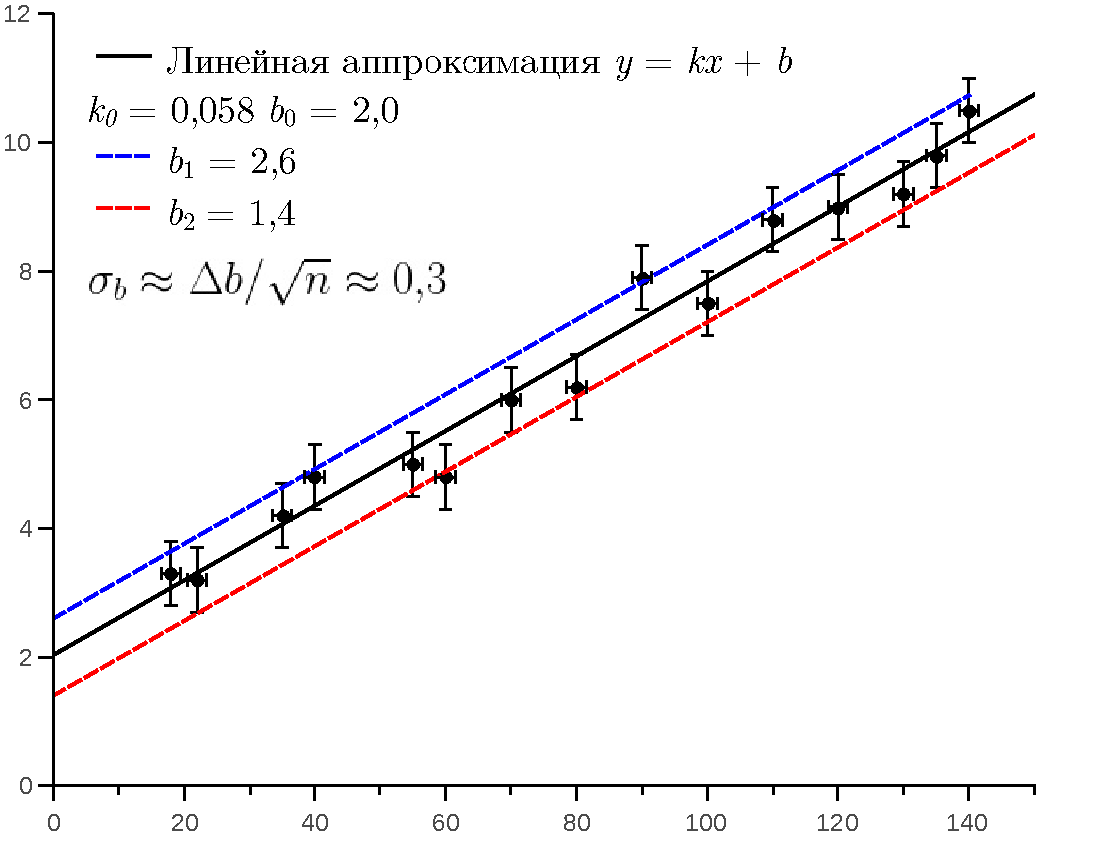
\includegraphics[width=1\linewidth]{images/graph1.pdf}%
\end{minipage}%
\begin{minipage}[t]{0.5\columnwidth}%
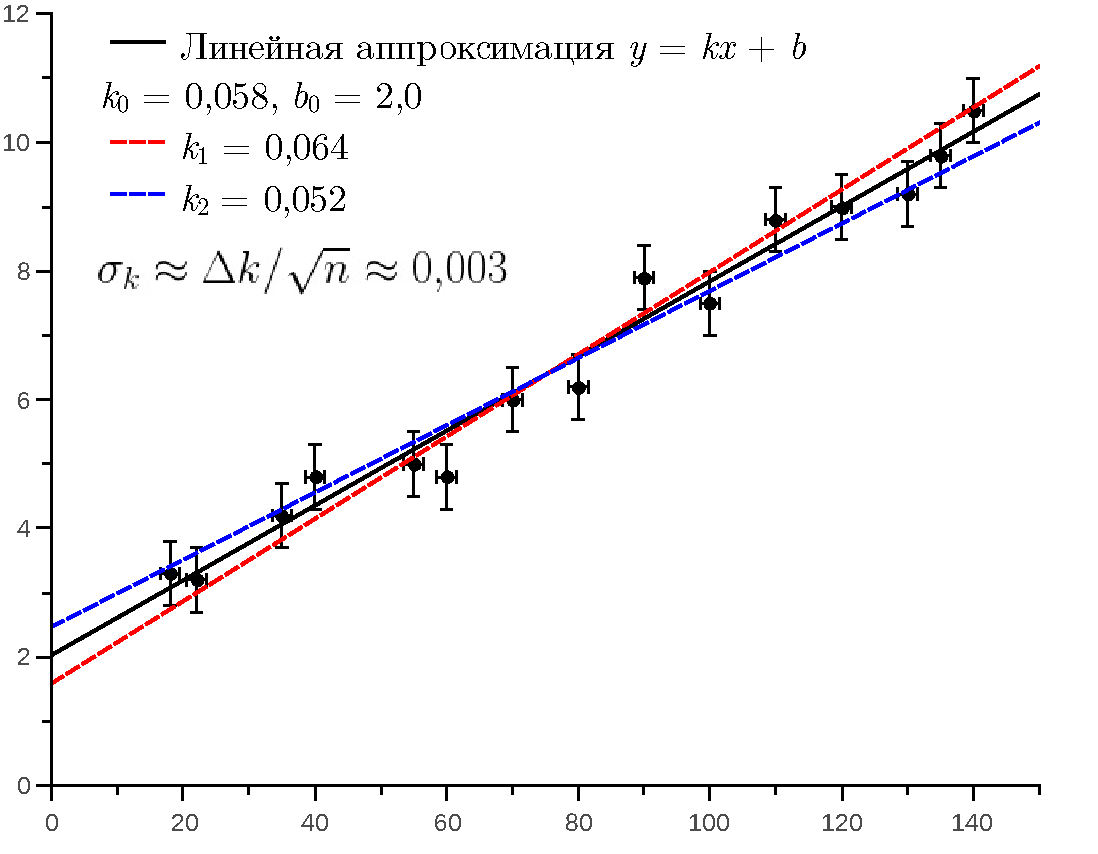
\includegraphics[width=1\linewidth]{images/graph2.pdf}%
\end{minipage}
\caption{Графический метод проведения прямой и оценки погрешностей}
\end{figure}

Самый простой и грубый метод --- провести наилучшую прямую
\textquote{от руки}. Этот метод, конечно, нестрогий,
но весьма наглядный. На практике к нему приходится часто прибегать
для грубой и быстрой оценки промежуточных результатов. Для этого нужно
приложить прозрачную линейку к графику так, чтобы по возможности кресты
всех экспериментальных точек находились максимально близко к проводимой
линии, а по обе стороны от неё оказалось примерно одинаковое количество
точек.

% \todo[author=ppv, inline]{Добавить отсылку к месту, где разбираются
% математические методы
% построения прямой}

Построив таким образом \textquote{наилучшую} прямую,
можно найти её параметры: угловой коэффициент $k$ и вертикальное
смещение $b$. Этим же способом можно грубо оценить ошибку определения
$k$ и $b$. Смещая линейку вертикально в пределах крестов погрешностей,
оценим погрешность $\delta b$. Аналогично, изменяя наклон линейки
относительно условного \textquote{центра масс}
экспериментального графика, получим оценку для погрешности углового
коэффициента $\delta k$. Если известно, что погрешности экспериментальных
точек $\left(\delta x,\,\delta y\right)$ имеют преимущественно случайный
характер, результат стоит разделить корень из числа точек:
$\sigma_{k}\approx\delta k/\sqrt{n}$,
$\sigma_{b}\approx\delta b/\sqrt{n}$ (для систематических погрешностей
так делать не стоит).

Эта же процедура позволяет проверить, является ли измеренная зависимость
в самом деле линейной: прямая должна пересекать большую часть (хотя
бы 2/3) крестов погрешностей. В противном случае можно предполагать
существенное отклонение экспериментальной зависимости от линейной
теоретической. Отметим, что если кресты погрешностей на графике не
отмечены, такой анализ провести затруднительно.

Существуют и аналитические методы подбора параметров (см. гл.~\ref{ch:estimate}),
минимизирующие отклонения экспериментальных точек от некоторой теоретической зависимости
(например, \emph{метод наименьших квадратов}). Студентам первого курса
рекомендуется осваивать их постепенно, по мере накопления опыта экспериментальной
работы.

\begin{figure}
    \centering
    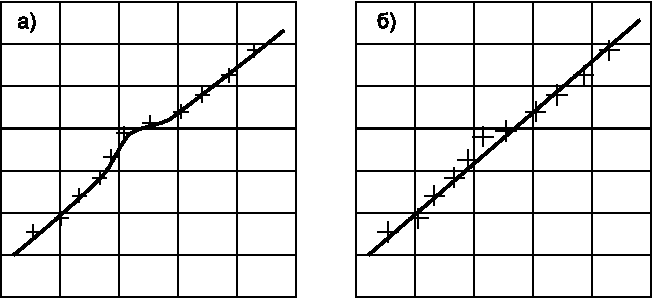
\includegraphics[width=0.8\linewidth]{errorbars.pdf}
    \caption{}
    \label{fig:graph-method}
\end{figure}

\example{На рис. \ref{fig:graph-method} изображены одни и те же
    экспериментальные точки при разных погрешностях измерений,
график \ref{fig:graph-method}а, несомненно,
указывает на нерегулярный ход изучаемой зависимости
(кривая линия). Те же данные при больших погрешностях опыта
(рис. \ref{fig:graph-method}б) успешно описываются прямой линией.
Без указания крестов погрешностей разделить эти два случая было
бы невозможно.}

\paragraph{Нелинейные зависимости.}

Если теория предсказывает \emph{нелинейную} функциональную зависимость
между величинами, часто можно сделать \emph{замену переменных} так,
чтобы результирующий график получался линейным.

Заметим, что аналитические методы позволяют подбирать параметры и для нелинейных
зависимостей. Хотя готовых формул для общего случая не существует, задача
легко решается численно --- и в большинстве современных программ обработки
данных это сделать не сложнее, чем построить наилучшую прямую.
Построение прямой является наиболее наглядным и позволяет проверить
\textquote{разумность} полученных результатов, сверив их с построением
\textquote{от руки}.

%Однако в учебной лаборатории такой подход использовать не рекомендуется.

\example{Высота и время падения
груза без начальной скорости в поле тяжести связаны соотношением
$y=\frac{1}{2}gt^{2}+y_{0}$.
Для того, чтобы получить линейную зависимость, можно построить график
в координатах $\left(y,t^{2}\right)$. По угловому коэффициенту наилучшей
прямой можно в таком случае вычислить ускорение свободного падения:
$k=\frac{1}{2}g$.}

\example{В термодинамике и химии часто встречается зависимость
    вида $y=Ce^{-a/x}$. Чтобы определить коэффициенты $C$ и $a$,
    можно построить график в координатах $(u,v)$, где $u=\ln y$ и
    $v=\frac{1}{x}$. В таком случае, как нетрудно видеть, $u=-av+\ln C$.}

Допускается использования программных пакетов для обработки линейных и нелинейных зависимостей при условии, что студент понимает все детали 
применяемой процедуры обработки.

\subsection{Рекомендации по оформлению графиков}

Основная цель использования графиков --- \emph{наглядность}
отображения результатов. В связи с этим к ним
предъявляются следующие требования:
\begin{itemize}
    \item график обязательно должен иметь подпись (заглавие) с кратким описанием его
содержания (графики --- это первое, на что обращает внимание читатель, еще до прочтения текста отчёта!);
\item подписи, данные и линии не должны быть нагромождены друг на друга
так, что препятствовало бы их чтению;
    \item оси на графике должны быть \emph{подписаны}: указаны буквенное
обозначение
величины и её единицы измерения; если величина безразмерна, указывается
\textquote{отн. ед.} (относительные единицы);
    \item на осях должны быть отмечены \emph{масштаб} и \emph{положение нуля};
масштаб обозначается несколькими отметками с подписанными значениями
и дополнительными малыми отметками без подписей; масштаб должен быть
удобным для чтения (использованы \textquote{круглые}
числа, делящиеся на 10, 5 или 2);
    \item масштаб осей и начало отсчёта должны быть выбраны так, чтобы
экспериментальные
данные занимали всю площадь листа, отведённую под график;
    \item если график строится не \textquote{от нуля}, это
следует подчеркнуть отдельно, например \textquote{разрывом}
оси;
    \item при необходимости сравнения данных из разных серий измерений, их
следует
размещать на одном графике, обозначая их разными символами или цветами;
    \item график с несколькими сериями данных должен быть снабжен \textquote{легендой},
в которой указано соответствие серий данных и их обозначений; экспериментальные
\textquote{точки} должны изображаться \emph{символами
конечных размеров} (позволяющими отличить их от случайных \textquote{пятен});
    \item точки не должны быть без необходимости соединены линиями; также не
нужно подписывать положение каждой точки графика (при необходимости
можно указать положение 1-2 \emph{особых} точек, если это не загромождает
график);
    \item все экспериментальные точки должны быть снабжены \emph{крестами
погрешностей},
размер которых соответствует инструментальной погрешности измерения
соответствующей величины (либо вычисленной по результатам косвенных
измерений); кресты погрешностей можно не отмечать, только если погрешности
малы (настолько, что они не будут видны на графике) или не известны;
    \item если теория предполагает некоторую (например, линейную) функциональную
зависимость, на график должна быть тонкой линией нанесена соответствующая
теоретическая кривая; расчёт параметров этой кривой (например, коэффициентов
МНК для линейной зависимости) должен проводиться отдельно в тексте
отчёта --- с указанием используемых методов и формул; результаты
таких расчётов и их погрешности указываются в легенде графика или
в подписи к нему;
    \item оптимальный размер графика --- от четверти до половины страницы
(при условии, что отчёт оформляется на страницах формата А4).
\end{itemize}

На рис.~\ref{fig:incorrect} приведён пример того, как \emph{не надо}
строить графики. В нём собраны наиболее типичные ошибки, совершаемые
студентами. Предлагаем читателю выявить их самостоятельно. Для сравнения
на рис.~\ref{fig:correct} изображён график для \emph{тех же данных},
выполненный с соблюдением изложенных выше указаний.
\begin{figure}[ht]
\begin{centering}
\includegraphics[width=9cm]{images/bad.png}
\par\end{centering}
\caption{\label{fig:incorrect}Пример неправильно построенного графика}
%     (график построен с использованием электронных таблиц LibreOffice Calc)
\end{figure}
\begin{figure}[ht!]
\begin{centering}
\includegraphics[width=8.5cm]{images/good.pdf}
\par\end{centering}
\caption{\label{fig:correct}Пример корректного графического представления
    данных}
% (график построен с использованием специализированного приложения
% для анализа и визуализации данных QtiPlot)
\end{figure}


\section{Некоторые типичные ошибки обработки данных}

\paragraph{Нахождение углового коэффициента по среднему от частного.}

Студент измеряет сопротивление резистора по зависимости $U\!\left(I\right)$.
Получив некоторое количество экспериментальных точек
$\left(I_{i},\,U_{i}\right)$,
и пользуясь законом Ома $R=U/I$, он вычисляет сопротивление для каждого
измерения $R_{i}=U_{i}/I_{i}$, а затем определяет сопротивление резистора
как среднее значение $R_{0}=\left\langle R_{i}\right\rangle =\frac{1}{n}\sum
R_{i}$.
Что не так с этим методом (результат-то получается вполне \textquote{разумным})?

\begin{longnote}
    Во-первых, применять процедуру усреднения можно только
    при повторении \emph{одного и того же} измерения. В данном случае значения
$R_{i}$
    относятся к \emph{разным} измерениям, так как параметры системы каждый раз
изменялись.
    Во-вторых, не была проверена линейность зависимости $U\left(I\right)$, то
есть
    справедливость закона Ома (ведь существуют и нелинейные элементы,
    для которых он не выполняется). В-третьих, даже если зависимость
    можно считать линейной, может оказаться так, что она не проходит через
    ноль (например, из-за сдвига нуля у вольтметра или амперметра) ---
    тогда формула $R_{i}=U_{i}/I_{i}$ не годится.
    И наконец, даже если выполнена линейность и зависимость проходит через
    ноль, вычисление таким способом чревато большими погрешностями. Нетрудно
    видеть, что среднее значение $\left\langle U_{i}/I_{i}\right\rangle $
    по сути есть среднее тангенсов углов наклона линий, проведённых из
    начала координат в экспериментальную точку. Как известно,
    функция $\tg x$ при $x>\pi/4$ очень резко возрастает (и стремится
    к бесконечности при $x=\pi/2$). В таком случае даже небольшое \textquote{шевеление}
    экспериментальной точки, особенно если она находится достаточно близко
    к оси ординат, может привести к резкому увеличению вклада этой точки
    в итоговый результат.

    Таким образом, \textquote{разумный} результат студента --- плод удачного стечения
многих
    обстоятельств. Правильный --- обоснованный и надёжный --- алгоритм
    нахождения сопротивления: построить график $U\left(I\right)$, убедиться
    в его линейности, и построить наилучшую прямую. 
    Угловой коэффициент этой прямой и будет наилучшей оценкой 
    для сопротивления резистора.
    \todo[inline]{Сделать рисунок}
\end{longnote}


\paragraph{Недооценка систематической погрешности.}
Студент измеряет сопротивление резистора, действуя по правильному
алгоритму, описанному выше. При измерениях используются вольтметр
и амперметр с классом точности $0{,}5$. Получив большое число экспериментальных
точек и построив наилучшую прямую методом наименьших квадратов (формула
(\ref{eq:MNK})), студент находит сопротивление (например, $R=5{,}555$~Ом)
и его погрешность по формуле (\ref{eq:MNK_sigma_k}), которая оказывается
равна $\sigma_{R}=0{,}003\;\text{Ом}.$ Окончательный результат измерения
записывается как $R=5{,}555\pm0{,}003\;\text{Ом}$.

Выходит так, что с помощью приборов, относительная погрешность которых
составляет $0{,}5\%$, получен на порядок более точный результат
$\varepsilon\approx0{,}05\%$.
Возможно ли такое?

\begin{longnote}
Ситуация эта вполне реальна и встречается в учебной лаборатории довольно часто.
Дело в
том, что метод наименьших квадратов позволяет оценить \emph{только
случайную ошибку} --- и она в самом деле может оказаться довольно мала. Однако
учебные приборы далеки от совершенства и их ошибка имеет в основном
\emph{систематический} характер. Поэтому в данном случае при записи конечного
результата
необходимо учесть систематическую ошибку, относительная величина которой по
составляет
не менее $0{,}5$\% (согласно классу точности прибора) и значительно превосходит
случайную. Результат эксперимента стоило бы записать как
$R=5{,}55\pm0{,}03\;\text{Ом}$.

Всё же, может статься и так, что инструментальные
ошибки наших вольтметра и амперметра имеют случайный характер, и мы
в самом деле добились кратного повышения точности за счёт многократных
повторений измерений (сколько нужно измерений, чтобы увеличить точность
на порядок?). Это нетрудно проверить, если заменить вольтметр или
амперметр на аналогичный и повторить опыты. Таким образом мы превратим
систематическую ошибку \emph{одного} прибора в случайную ошибку
\emph{множества}
приборов. Если отклонение нового результата от исходного значительно
превысит величину $\pm0{,}003$~Ом, гипотеза о случайности инструментальной
ошибки будет опровергнута, то есть погрешность отдельного прибора
действительно имеет в основном систематический характер.\par
\end{longnote}

\paragraph{Аппроксимация полиномом.}
Студент получает набор экспериментальных данных $\left\{ x_{i},y_{i}\right\} $,
которые по теории должны ложиться на прямую. Нанеся точки на график,
студент видит, что на прямую они ложатся не очень хорошо (см.
рис.~\ref{fig:approx}а).
Для того, чтобы точки лучше ложились на график, студент решает использовать
функцию аппроксимации полиномом (например, квадратичным), имеющуюся
в наличии во всех электронных таблицах и программах обработки данных.
Можно ли так делать?

\begin{figure}[h]
\begin{minipage}[t]{0.49\columnwidth}%
\begin{center}
\includegraphics[width=1\linewidth]{images/x2.pdf}
\par\end{center}
\begin{center}
а)
\par\end{center}%
\end{minipage}%
\begin{minipage}[t]{0.49\columnwidth}%
\begin{center}
\includegraphics[width=1\linewidth]{images/x2b.pdf}
\par\end{center}
\begin{center}
б)
\par\end{center}%
\end{minipage}
\caption{\label{fig:approx}Примеры аппроксимации данных: а)~сплошная линия
--- линейная аппроксимация, пунктир --- квадратичная
аппроксимация; б)~сплошная линия --- линейная аппроксимация
по нескольким начальным точкам, пунктир --- аппроксимация
полиномом высокой степени.}
\end{figure}

\begin{longnote}
    Ответ на вопрос зависит от того, какую цель преследует
    студент. Если цель --- добиться того, чтобы \textquote{точки лучше ложились на график}, то всё сделано правильно.
    Если говорить \textquote{по-научному} ---
    это попытка решить задачу \emph{интерполяции}
    экспериментальных данных: по ограниченному набору $\left\{
x_{i},\,y_{i}\right\} $
    получить аналитическую функцию $y=f\!\left(x\right)$, позволяющую
    рассчитывать значения $y$ при произвольном $x$. В учебном практикуме
    это может быть, например, задача построения калибровочного графика.
    В таком случае можно лишь дать практический совет --- стараться
    использовать для интерполяции полином \emph{как можно
    меньшей степени} (дело в том, что при слишком большой
    степени функция почти наверняка станет сильно немонотонной, а это
    вовсе не то, что хочется иметь в качестве результата интерполяции,
    см. рис.~\ref{fig:approx}б).

    Однако ни в одной лабораторной работе курса общей
    физики задача интерполяции не является основной целью работы! Как
    правило, цель --- проверить теоретические закономерности
    и измерить физические характеристики системы. Если нет теории,
предсказывающей
    и объясняющей квадратичную зависимость, проделанная студентом процедура
    \emph{бесполезна}, поскольку вычисленным коэффициентам полинома
затруднительно
    приписать физический смысл.

    Правильно было бы в такой ситуации выявить, на каком
    участке зависимости линейный закон \emph{выполняется},
    оценить его границы, и по нему построить наилучшую прямую (сплошная
    линия на рис.~\ref{fig:approx}б). Для участка, отклоняющегося от
    предсказываемой линей зависимости, следует теоретически проанализировать
    причины отклонения и по возможности предложить уточнение теории. Возможно,
    стоит ожидать не квадратичное, а кубическое отклонение? Различить
    их на ограниченном наборе данных с большими погрешностями невозможно!
    Имея достаточное количество точек предложенную теорию можно проверить
    и лишь после этого аппроксимации более сложной функцией можно придать
    физический смысл.
\end{longnote}
